\documentclass[border=2pt]{standalone}
\usepackage[T1]{fontenc}
\usepackage{mathptmx}
\usepackage{tikz}
\usetikzlibrary{arrows.meta,positioning,fit,calc,shapes.geometric,backgrounds}
\usepackage{siunitx}
\tikzset{
  >={Stealth[length=1.8mm]},
  blk/.style={draw, thick, minimum height=11mm, text width=16mm, align=center, font=\scriptsize, inner sep=1.5pt, fill=white},
  lab/.style={font=\scriptsize, align=center},
  every picture/.style={line width=0.6pt},
}

\begin{document}
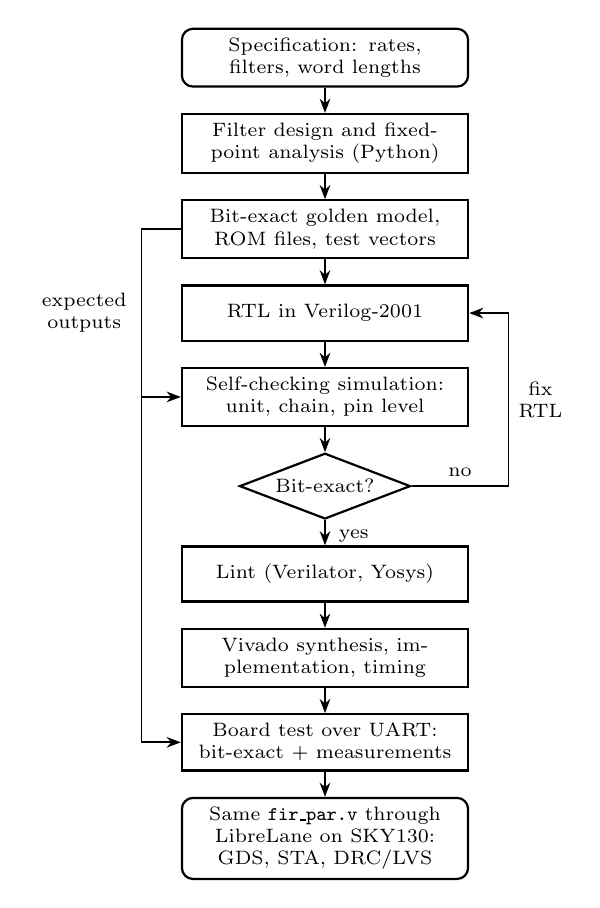
\begin{tikzpicture}[node distance=3.2mm,
  st/.style={draw, thick, text width=34mm, minimum height=7mm, align=center, font=\scriptsize, fill=white},
  dec/.style={draw, thick, diamond, aspect=2.6, inner sep=0.5pt, align=center, font=\scriptsize, text width=16mm}]
\node[st, rounded corners] (spec) {Specification: rates, filters, word lengths};
\node[st, below=of spec] (py) {Filter design and fixed-point analysis (Python)};
\node[st, below=of py] (gold) {Bit-exact golden model, ROM files, test vectors};
\node[st, below=of gold] (rtl) {RTL in Verilog-2001};
\node[st, below=of rtl] (tb) {Self-checking simulation: unit, chain, pin level};
\node[dec, below=of tb] (eq) {Bit-exact?};
\node[st, below=of eq] (lint) {Lint (Verilator, Yosys)};
\node[st, below=of lint] (viv) {Vivado synthesis, implementation, timing};
\node[st, below=of viv] (hil) {Board test over UART: bit-exact + measurements};
\node[st, below=of hil, rounded corners] (asic) {Same \texttt{fir\_par.v} through LibreLane on SKY130: GDS, STA, DRC/LVS};
\foreach \a/\b in {spec/py,py/gold,gold/rtl,rtl/tb,tb/eq,eq/lint,lint/viv,viv/hil,hil/asic} \draw[->] (\a) -- (\b);
\node[lab, right=0.5mm of eq.south, anchor=north west] {yes};
\coordinate (xr) at ($(rtl.east)+(5mm,0)$);
\draw[->] (eq.east) -- node[lab, above]{no} (eq.east -| xr) |- (rtl.east);
\node[lab, right] at ($(xr)!0.5!(xr |- eq.east)$) {fix\\RTL};
\draw[->] (gold.west) -- ++(-5mm,0) |- node[lab, pos=0.25, left, text width=12mm]{expected outputs} (tb.west);
\draw[->] (gold.west) ++(-5mm,0) |- (hil.west);
\end{tikzpicture}
\end{document}
